\documentclass{beamer}
%\documentclass[notes]{beamer}
%\documentclass[notes=only]{beamer}
\usepackage{xeCJK}
\setCJKsansfont[Path=/System/Library/Fonts/Supplemental/]{Songti.ttc}
\usepackage[dvipsnames]{xcolor}
\usepackage{multicol,multirow,lipsum,caption,graphicx}
\usepackage{mathtools, amsmath,booktabs,verbatim,tikz} 
\usetikzlibrary{shapes.geometric, arrows,positioning,matrix,calc}
\usepackage{booktabs, makecell, amsmath,afterpage}
\usepackage{tikz,tabularx, adjustbox}
\usepackage{booktabs, multicol,multirow, makecell, afterpage}
\usepackage{subcaption}
\usepackage{algorithm}
\usepackage{algpseudocode}
%\usepackage{mathptmx}

\newcommand\scalemath[2]{\scalebox{#1}{\mbox{\ensuremath{\displaystyle #2}}}}

\usetheme[progressbar=frametitle]{metropolis}
\setbeamertemplate{frame numbering}[fraction]
\useoutertheme{metropolis}
\useinnertheme{metropolis}
\usefonttheme{metropolis}
\usecolortheme{spruce}
\setbeamercolor{background canvas}{bg=white}

% Top left Position of a logo in beamer
\titlegraphic { 
\begin{tikzpicture}[overlay,remember picture]
\node[left=0.0cm] at (current page.28){
    
\includegraphics[width=2.8cm]{wuhan.png}
};
\node[left=-4cm] at (current page.151){
    
\includegraphics[width=3.5cm]{kit.png}
};
\end{tikzpicture}
}

\usepackage{textpos}
\addtobeamertemplate{frametitle}{}{
	\begin{textblock*}{15mm}(0.86\textwidth,-1.1cm)
		
\includegraphics[width=2.5cm]{kit_logo.png}
	\end{textblock*}
	}	

%\title{无锡太湖学院物联网工程学院面试汇报}
\title{第二届崇真青年学者学术沙龙报告\\
\large 计算机与人工智能学院 \\
\normalsize 武汉纺织大学}
\author{汇报人:张辉耀 }
\date{汇报时间:2022年4月23号}
\setbeamertemplate{itemize/enumerate body begin}{\large}

\DeclarePairedDelimiter\Floor\lfloor\rfloor
\DeclarePairedDelimiter\Ceil\lceil\rceil
\begin{document}
\begin{frame}
    \titlepage
\end{frame}
\note{尊敬的各位老师好,我叫张辉耀,首先很荣幸能够参加此次面试,
也感谢各位老师在星期天的下午,这样一个时间,听我汇报,
下面我就我的教育背景做一个简单的介绍。}

\begin{frame}{教育背景}
	\begin{itemize}
		\item 本科 \textcolor{white}{e} 大连工业大学 \textcolor{white}{e}
			2011.09-2015.07
		\item 硕士 \textcolor{white}{e} 上海东华大学  \textcolor{white}{e}
			2015.09-2018.03
			\begin{itemize}
				\item 专业:数字化纺织工程
				\item 研究内容:椭圆傅立叶和凸包算法在人体建模的应用 
			\end{itemize}
		\item 博士 \textcolor{white}{e} 日本京都工艺纤维大学 \textcolor{white}{e}
			2018.09-2022.03
			\begin{itemize}
				\item 专业:先端纤维学
				\item 研究内容:遗传算法和神经网络在材料科学的应用 
			\end{itemize}
	\end{itemize}
\end{frame}

\note{我本科毕业于大连工业大学,研究生就读于上海东华大学纺织学院, 所学的专业是数字化纺织工程,
在读研期间,接触到计算科学在纺织服装和材料领域的应用,于是对计算科学和数学产生了
强烈的兴趣。
我在研究生期间的主要工作是使用椭圆傅立叶和凸包算法解决了一些三维人体建模的问题。
研究生毕业以后,由于当时导师的推荐和国家留学基金委的资助,来到日本京都
工艺纤维大学攻读博士,并于上个月取得博士学位。}

\begin{frame}{研究契机}
	\begin{columns}
		\begin{column}{0.6\textwidth}
			\begin{figure}
				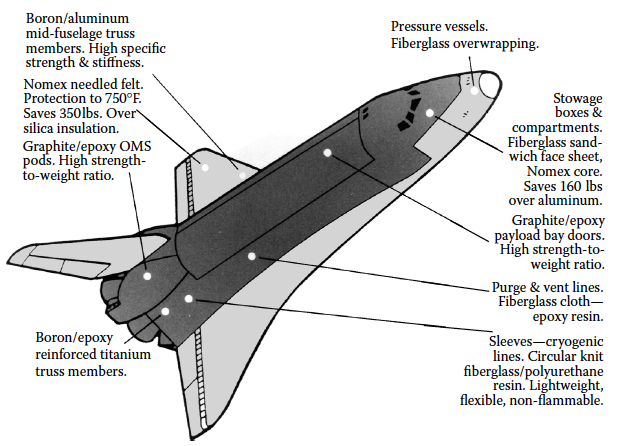
\includegraphics[width=1.0\linewidth]{fig/part0/space-shuttle.png}
				\caption{层合材料的应用一 (Graphic courtesy of M.C. Gill Corporation,
				http://www.mcgillcorp.com.)}
			\end{figure}
		\end{column}
		\begin{column}{0.4\textwidth}
			\begin{figure}
				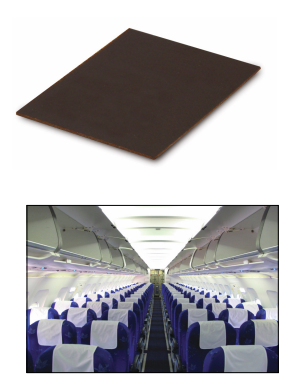
\includegraphics[width=1.0\linewidth]{fig/part0/laminate_product.png}
				\caption{层合材料的应用二 (https://www.thegillcorp.com)}
			\end{figure}
		\end{column}
	\end{columns}
\end{frame}

\note{ 
1. Composite material gains more and more influence in commerical industry
because of its excellant mechanic performance in stiffness, stength etc., over
conventional materials.  
1. 层合材料由于其在强度和刚度等方面优良的性质广泛的应用于社会生活的方方面面。
在这里给出两个例子

2. Here are two examples of the use of them, the first one
is used in the space shuttle, for the main body of the space shuttle, down the
red arrow, the main reason it was chosen for weight saving and for small
mechanical and thermal deflections. 
2. 图一是复合材料应用在宇宙飞船上,在这里使用复合材料的主要原因是它能够在保持
强度的同时降低飞船自身的重量,并且在受到高温和强力冲击的时候具有较小的变形。

3. The second example is the use in the air plane,  which is because of its high
mechanical strength, heat resistant, and very low smoke evolution in a smoke.
图二是复合材料使用在飞机上,在这里使用复合材料的原因是因为复合材料的热阻效果,
和其在燃烧的时候产生 的烟雾颗粒较小。
}

\begin{frame}{什么是层合材料?}
    \begin{columns}[c]
		\begin{column}{0.6\textwidth}
			\begin{figure}
			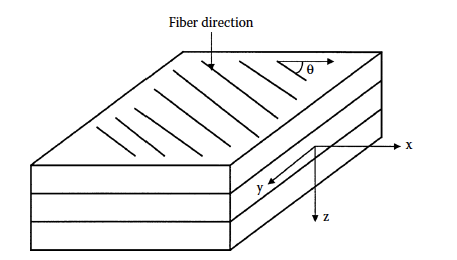
\includegraphics[width=0.85\linewidth]{fig/part0/Schematic_of_a_laminate.png}
			\caption{ 层合材料结构图 (来源: Autar k. kaw 2006)}
			\end{figure}
		\end{column}
		\begin{column}{0.4\textwidth}
			\begin{figure}
			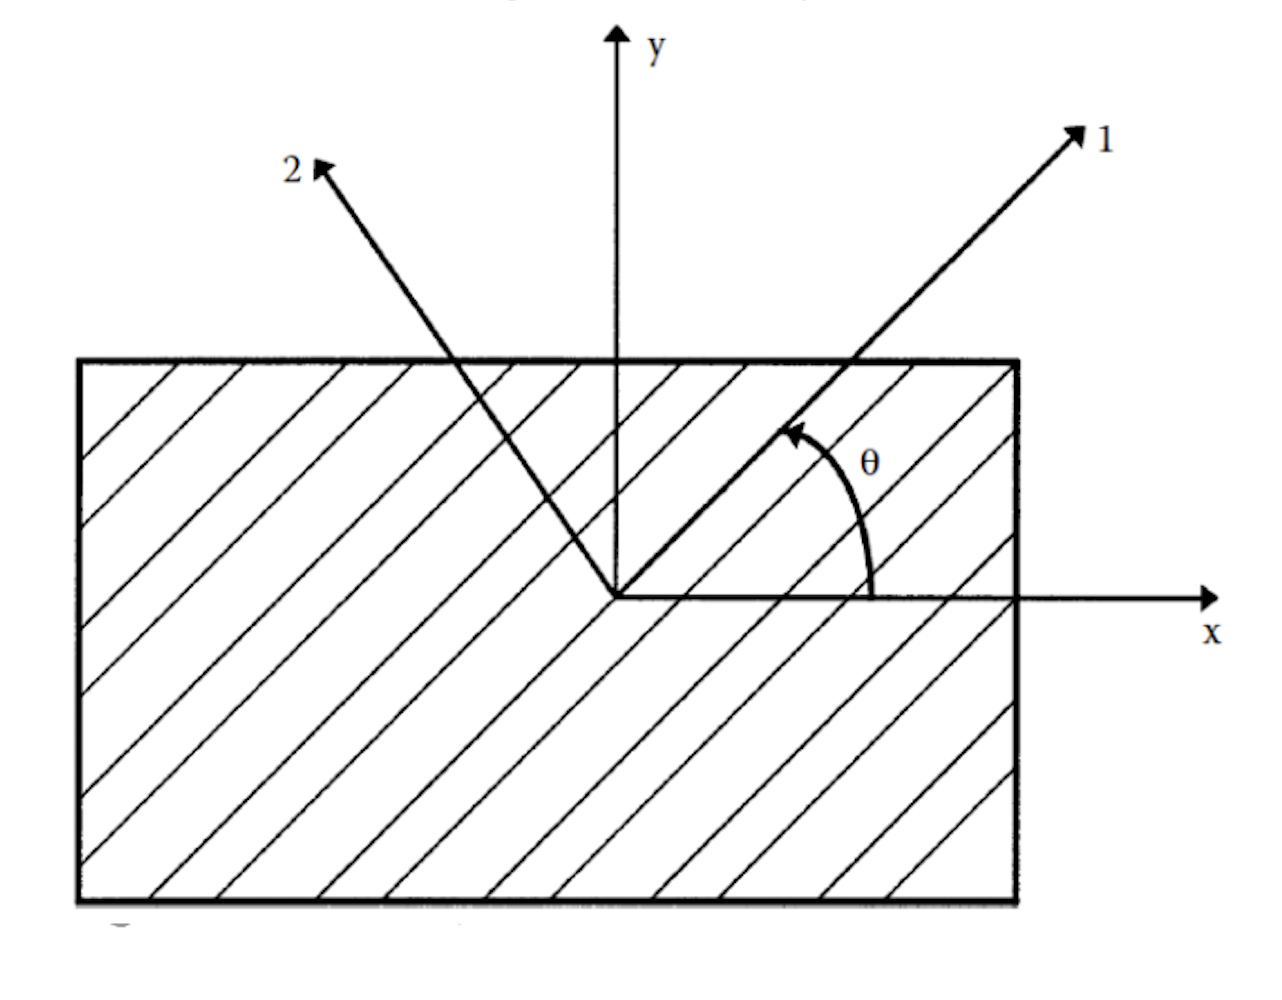
\includegraphics[width=1\linewidth]{fig/local.png}
			\caption{ 层合材料的断面图 (来源: Autar k. kaw 2006)}
			\end{figure}
		\end{column}
	\end{columns}
\end{frame}
\note{ 
1. A laminate is an assembly of layers of composite materials which can be
joined to provide required engineering properties.  Figure 1 is the schematic of
a laminate. 
层合板是由复合材料粘结而成的能够满足指定工程强度的一种特殊复合材料。
2. For each layer, its properies is determined by several variables: the
thickness of the layer, the fiber orientation, and engineering properites of the
material. The properitis of a laminate is determined by the combination of these
layers.  
图三是层合材料的结构图, 对于层合材料各层材料而言,铺层的角度,厚度和材料可以是
不同的,所以层合材料的设计有着极大的自由度。

A question arises from this is how to determine the strength of a laminate.
}


\begin{frame}{怎样设计?}
			\begin{itemize}
					\item 层合材料设计:
				\begin{itemize}
					\item 目标:强度 
					\item 约束条件:重量,成本等
					\item 变量: 铺层角度,铺层数,材料等
				\end{itemize}
				\item 本质上是受约束离散变量的优化设计问题
			\end{itemize}
\end{frame}

\note{
1. But how to design it.
2. In practice, we need to tailor the structure of a laminate 
material to satisfy engineering requirements. such as the weight and cost.  
3. the layout of this  sequence is determined by several variables, the ply
thickness, the number of layers, the ply oritentation. And all these variables
are discrete in practice.  So in nature the design of laminated composite
material is a constrained optimization with discrete variables.

在生产中,使用的层合材料除了需要满足工程强度的要求以外,还对生产成本和材料本身的
质量要求。
层合材料的强度取决于层合板的层数,铺层角,层合材料等。以上这些决定层合板强度的变量
都是离散的,因此层合材料的设计是一个受约束的离散变量的优化问题。
}


\begin{frame}{研究方法} 
	\begin{columns}
		\begin{column}{0.65\textwidth}
			\begin{itemize}
				\item  1. 构造目标函数 $f(x)$.
				\item  2. 为满足约束条件,添加惩罚项
					$\phi_1(x),\phi_2(x),\cdots, \phi_n(x)$ 
				\item  3. 重新构造目标函数

					$f(x)+c_1\phi_1(x)+c_2\phi_2(x)+ \cdots + c_n\phi_n(x)$
			\end{itemize}
		\end{column}
		\begin{column}{0.35\textwidth}
			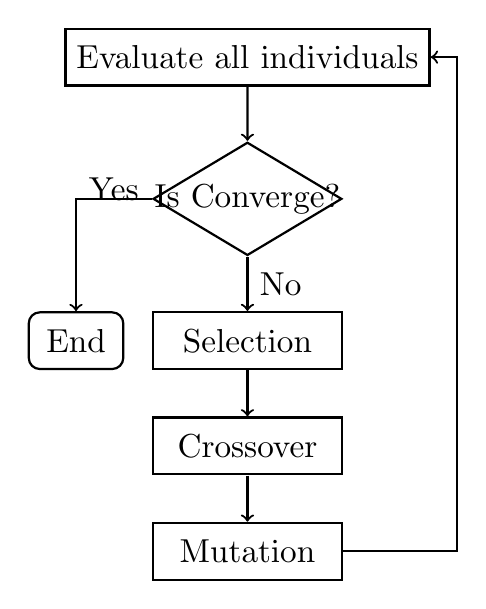
\begin{tikzpicture}[thick, scale=1.2, every node/.style={transform shape}]
	\tikzstyle{startstop} = [rectangle, rounded corners, minimum width=1.0cm,minimum height=0.6cm, text centered, draw=black]
	\tikzstyle{io} = [trapezium, trapezium left angle=70, trapezium right angle=110, minimum width=2cm, minimum height=0.6cm, text centered, draw=black]
	\tikzstyle{process} = [rectangle, minimum width=2cm, minimum height=0.6cm, text centered, draw=black]
	\tikzstyle{decision} = [diamond,minimum width=2cm, minimum height=1.2cm, draw=black]
	\node (fitness) [process] {Evaluate all individuals};
	\node[yshift=-0.5cm] (decision) [decision, below of=fitness] {} node at (decision.base) {Is Converge?};
	\node[yshift=-0.5cm] (selection) [process, below of=decision] {Selection};
	\node (crossover) [process] at ($(selection.south)+(0,-0.8cm)$) {Crossover};
	\node (mutation) [process] at ($(crossover.south)+(0,-0.8cm)$)  {Mutation};
	\node (end) [startstop] at ($(selection.west)+(-0.8cm,0cm)$) {End};

	\draw [->] (fitness) -- (decision);
	\draw [->] (decision.south) -- (selection.north) node[auto=left,pos=0.5]{No};
			   \node at ($(decision.west)+(-0.4cm, 0.1cm)$) {Yes};
	\draw [->] (selection.south) -- (crossover.north);
	\draw [->] (crossover.south) -- (mutation.north);
	\draw [->] (decision.west) -| (end.north);
	\draw [->] (mutation.east) -- ($(mutation.east)+(1.2cm,0cm)$) |-
		(fitness.east);
\end{tikzpicture}

		\end{column}
	\end{columns}
\end{frame}

\note{
对于离散变量的优化问题可以使用遗传算法进行解决,因为其不需要变量是连续的。
直接使用遗传算法来解决层合材料的设计问题方法如下:
1. 构造目标函数
2. 为满足约束条件,添加相应的惩罚项到目标函数
3. 重新构造目标函数
但是这种做法会有两个问题:
但是遗传算法是为了无约束的目标优化提出来的,对目标函数的重新构造会影响遗传算法的
性能,
而且每次模拟只能得到一个结果,并且这个结果跟重新构造目标函数系数的系数有关。

	One of the most natural way to solve this problem is to adopt genetic
algorithm, because it doesn't require the variable to be continuous. 
This classical method works in the following step 
1. formulate the objective function. 
2. append all the constraints to the objective function as punishment items
3. reformulate the objective function.
In this formula, the coefficient c subscript 1 is coefficient whose value is from 0 to 1.
The drawback of this method is that genetic algorithm is proposed for unconstrained problem, you have to reformulate the objective function.
}



\begin{frame}{研究方法}
	\begin{columns}
		\begin{column}{0.6\textwidth}
			\begin{itemize}
				\item  1. 构造目标函数 $f(x)$.
				\item  2. 为满足约束条件,在群体中维护不同的子群 
				\item  3. 不改变目标函数 $f(x)$.
			\end{itemize}
		\end{column}
		\begin{column}{0.4\textwidth}
			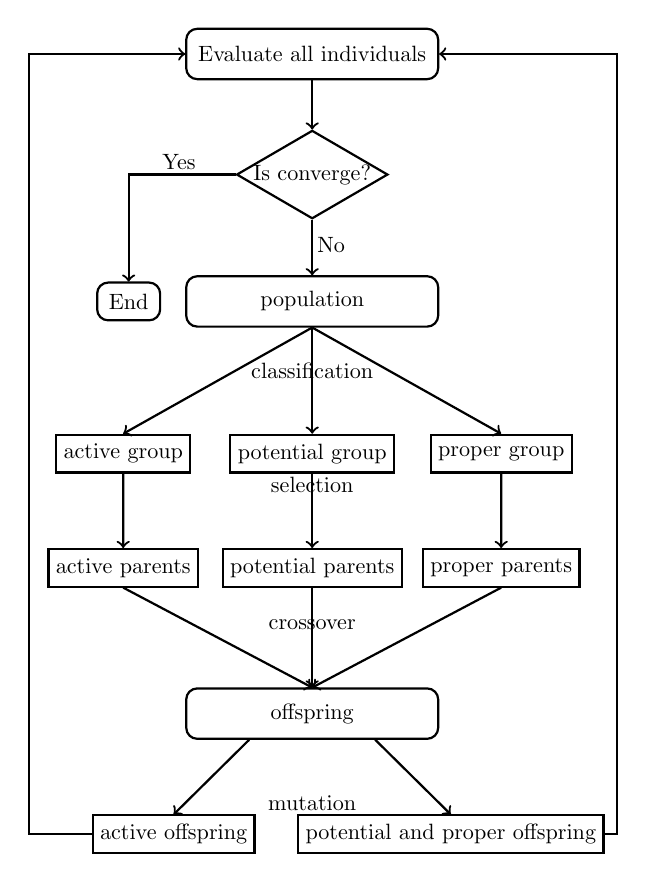
\begin{tikzpicture}[thick, scale=0.8, every node/.style={transform shape}]
	\tikzstyle{startstop} = [rectangle, rounded corners, minimum width=1.0cm,minimum height=0.6cm, text centered, draw=black]
	\tikzstyle{rec} = [rectangle,rounded corners, minimum width=4cm, minimum height=0.8cm,
	text centered, draw=black]
	\tikzstyle{subgroup} = [rectangle, minimum width=1.5cm, minimum height=0.6cm,
	text centered, draw=black]
	\tikzstyle{bigsubgroup} = [rectangle, minimum width=2.5cm, minimum height=0.6cm,
	text centered, draw=black]
	\tikzstyle{decision} = [diamond,minimum width=2.4cm, minimum height=1.4cm, draw=black]
	% population
	\node (evaluate) [rec] {Evaluate all individuals};
	\node (decision) at ($(evaluate.south)+(-0cm, -1.5cm)$)   [decision] {} node at (decision.base) {Is converge?};
	\node at  ($(decision.south)+(0.3cm, -0.4cm)$) {No};
	\node at  ($(decision.west)+(-0.9cm, 0.2cm)$) {Yes};
	\node (population) at ($(decision.south)+(-0cm, -1.3cm)$) [rec] {population};
	\node (end) at ($(population.west)+(-0.9cm, 0cm)$) [startstop] {End};
	% active group
	\node (active_group_1) at ($(population.south)+(-3cm, -2.0cm)$) [subgroup]
		{active group};
		\node (active_group_2) at ($(active_group_1.south)+(0cm, -1.5cm)$)
			[subgroup] {active parents};
		\draw[->] (decision.west) -| (end.north);
		\draw[->] (population.south) -- (active_group_1.north);
		\draw[->] (active_group_1.south) -- (active_group_2.north);
		% potential group
		\node (potential_group_1) at ($(population.south)+(0cm, -2.0cm)$) [subgroup]
				{potential group};
		\node (potential_group_2) at ($(potential_group_1.south)+(0cm, -1.5cm)$)
			[subgroup] {potential parents};
		\draw[->] (evaluate.south) -- (decision.north);
		\draw[->] (decision.south) -- (population.north);
		\draw[->] (population.south) -- (potential_group_1.north);
		\draw[->] (potential_group_1.south) -- (potential_group_2.north);
		\node at ($(potential_group_1.north)+(0cm, 1.0cm)$) {classification };
		\node at ($(potential_group_2.north)+(0cm, 1.0cm)$) {selection};
		% proper group
		\node (proper_group_1) at ($(population.south)+(3cm, -2.0cm)$) [subgroup]
			{proper group};
		\node (proper_group_2) at ($(proper_group_1.south)+(0cm, -1.5cm)$)[subgroup]
			{proper parents};
		\draw[->] (population.south) -- (proper_group_1.north);
		\draw[->] (proper_group_1.south) -- (proper_group_2.north);
		% crossover
		\node (after_cross_over) at ($(potential_group_2.south)+(0cm, -2.0cm)$) [rec] {offspring};
		\node  at ($(after_cross_over.north)+(0cm, 1.0cm)$)  {crossover};
		\draw[->] (active_group_2.south) -- (after_cross_over.north);
		\draw[->] (potential_group_2.south) -- (after_cross_over.north);
		\draw[->] (proper_group_2.south) -- (after_cross_over.north);
		% mutation
		\node (active_group_3) at ($(after_cross_over.south)+(-2.2cm, -1.5cm)$)
			[subgroup] {active offspring};
		\node at ($(after_cross_over.south)+(0cm, -1.0cm)$) {mutation};
		\draw[->] ($(after_cross_over.south)+(-1cm,0cm)$)--(active_group_3.north);
		\node (poteni_and_prop) at ($(after_cross_over.south)+(2.2cm, -1.5cm)$)
			[bigsubgroup] {potential and proper offspring};
		\draw[->] ($(after_cross_over.south)+(1cm,0cm)$)--(poteni_and_prop.north);

		% final draw
		\draw[->] (poteni_and_prop.east) --($(poteni_and_prop.east) + (0.2cm,0cm)$) |- (evaluate.east);
		\draw[->] (active_group_3.west) -- ($(active_group_3.west) + (-1cm,0cm)$)
			|- (evaluate.west);
		\end{tikzpicture}

		\end{column}
	\end{columns}
\end{frame}

\note{
	为了解决以上这两个问题,对传统的遗传算法进行改进。
	
	1. first, classify the population into three different groups according to the
	constraints, active group, potential group and proper group. we will explain
	these terminology later.
	2. second, the mutation operator for active group and potential, proper
	group is different. For the active group, the mutation follows the
	traditional pattern; we will adopt new mutation technique for the potential
	and proper group.
	第二个改进是引入了自适应的演化算子,为潜在子群和合格子群。
	基于这两个techique,我们可以在不重新构造目标函数的前提下,完成受约束离散变量的优化
 }

\begin{frame}{定义}
		\begin{itemize}
			\item
				活跃个体和活跃子群:如果一个个体的约束值远小于约束条件,那么我们称该个体为活跃个体,
				该个体所在的子群为活跃子群。
			\item
				潜在个体和潜在子群:如果一个个体的约束值小于或者接近约束条件,那么我们称该个体为潜在个体,
				该个体所在的子群为潜在子群。
			\item
				合格个体和合格子群:如果一个个体的约束值满足约束条件,那么我们称该个体为合格个体,
				该个体所在的子群为合格子群。
		\end{itemize}
\end{frame}

\note{
	这是我们提出的改进遗传算法中的一些定义。

	Here are some definition and terminology:
The role of different group is different. The role of active group is to
maintain the diversity of the mating pool. The role of potential group is to
find possible solutions. In the proper group, they are  the individual that we want.}



\begin{frame}{自适应变异算子}
		$\text{md} = [CT_1, \cdots, CT_{n-1}, CT_n] -  [ICV_1, \cdots, ICV_{n-1},
		ICV_n]$ \\
		\begin{itemize}
			\item  md 表示变异向量 
			\item  $CT_i$ 表示第i个约束条件,比如质量,强度等。
			\item  $ICV_i$ 表示当前个体的相应的约束值。
		\end{itemize}

		\begin{equation}
			\text{长度变异算子} =  
			\left\{
				\begin{array}{l}
					  LMC*[0, \sum_{i=1}^{N}{md_i}]  \text{ if $\sum_{i=1}^{N}{md_i} > 0$} \\
					  LMC*[\sum_{i=1}^{N}{md_i}, 0]  \text{ if $\sum_{i=1}^{N}{md_i} < 0$} \\
				  \end{array} 
				  \right.
		\end{equation}
		\begin{equation}
			\text{角度变异算子} = 
				\left\{
					\begin{array}{l}
					0.5, \text{ AM = }[0,AMC \sum_{i=1}^{N}{(|CT_i-CV_i|)}] \\ 
					0.5, \text{ AM = }[ AMC \sum_{i=1}^{N}{(-|CT_i-CV_i|)},0] \\
					\end{array}
					\right.
		\end{equation}
\end{frame}

\note{
	第二个technique是自适应变异算子,它的意思就是个体能够根据自身的约束值
	和约束条件的关系调整演化的方向和速度。
	我们是通过以下的方式设计了两个变异算子,长度变异和角度变异:
	1. 根据个体的自身约束值和约束条件,得到一个变异向量
	2. 根据变异向量调整层合材料的角度变异和角度变异。
}


\begin{frame}{研究成果}
	\begin{center}
		\begin{itemize}
			\item Huiyao Zhang, Atsushi Yokoyama. 2021. A Technique for Constrained Optimization of Cross‑ply Laminates Using a New
				Variant of Genetic Algorithm. International Journal of Advanced Computer Science and Applications, 12(6): 760‑767.
			\item Huiyao Zhang, Atsushi Yokoyama. 2022. Optimum Design of Laminated Composites for Minimum Thickness by a Variant
				of Genetic Algorithm. Journal of Textile Engineering(accepted)
		\end{itemize}
	\end{center}
\end{frame}

\note{
	使用改进的遗传算法解决了在多个层合材料优化设计的问题,在计算机和材料的期刊上分别
	发表有学术论文。
}




\begin{frame}{问题二: 如何预测层合材料的强度? }
	\begin{center}
		\begin{figure}
			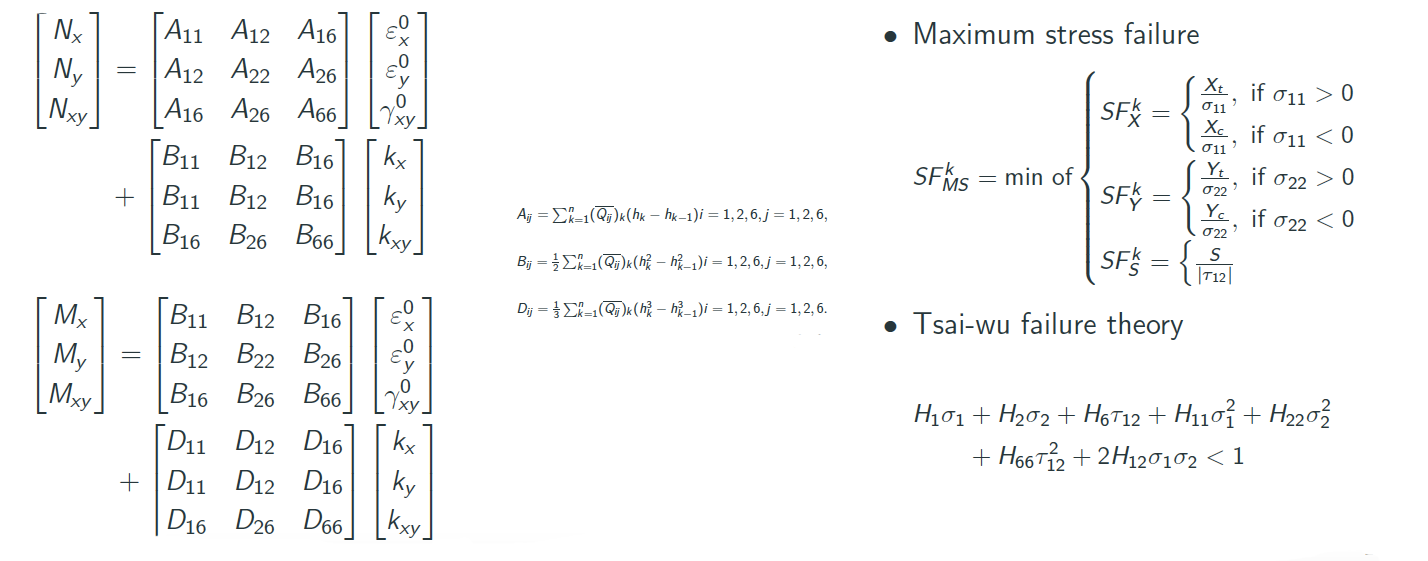
\includegraphics[width=1\textwidth]{fig/part3/formula_for_stenght_calculation.png}
		\end{figure}
	\end{center}
\end{frame}

\note{
	我博士期间研究的第二个问题呢
    我们可以使用这个幻灯片中的公式来计算层合材料的强度,这些公式有一个名字叫做,
	经典的层合理论和纤维失效理论。它本质上是一种解析的方法,根据经典的力学模型计算应力和应变来预测材料的强度。
	这种方法存在的一个问题是,她的步骤比较繁琐,而且这个算法的时间复杂度比较高,因为包含了
	大量的矩阵乘法和积分的运算。因此,我尝试使用使用数据驱动的方法,也就是神经网络来预测
	复合材料的强度。

Another problems arises from a laminate is the the strength prediction.
	The traditional way of doing this follows a two-step precedure: first,
	calculate the stress and strain within the laminated composite material by
	using of classical lamination theory. Second use failure theory to check the
	corresponding material failure or not. The first drawback of this method is
	that the computation cost is high because of the involvment of matrix
	multplication and interal operation and interal operation.  There we propose
	to use evolutionary artificial neural network to predict the strenght of
	angle ply laminate.}

\begin{frame}{如何设计网络的拓扑结构?}
	
\begin{figure}
	\begin{center}
\begin{tikzpicture}
[ plain/.style={ draw=none, fill=none, }, remember picture, net/.style={ matrix of nodes, nodes={ draw, circle,
    inner sep=7.5pt
    },
  nodes in empty cells,
  column sep=-10.5pt,
  row sep=0.8cm
  }
]
%\draw[help lines] (-3cm,-6cm) grid (6cm,3cm);
\matrix[net] (mat)
{
              & |[plain]| &           & |[plain]|  &           & |[plain]| &           &  |[plain]|      &               \\
    |[plain]| &           & |[plain]| &            & |[plain]| &           & |[plain]| &                 & |[plain]|     \\ 
    |[plain]| & |[plain]| &           & |[plain]|  &           & |[plain]| & 	  	   &  |[plain]|      & |[plain]|     \\ 
  };

  \node at ($(mat-1-1.west)+(-16pt,0)$) {输入层: };
  \node at ($(mat-2-2.west)+(-24pt,0)$) {隐藏层:};
  \node at ($(mat-3-2.west)+(-24pt,0)$) {输出层:};
  \node at (mat-1-1.base) {$i_1$};
  \node at (mat-1-3.base) {$i_2$};
  \node at (mat-1-5.base) {...};
  \node at (mat-1-7.base) {$i_{n-1}$};
  \node at (mat-1-9.base) {$i_{n}$};
  \node at (mat-2-2.base) {$h_1$};
  \node at (mat-2-4.base) {$h_2$};
  \node at (mat-2-6.base) {$...$};
  \node at (mat-2-8.base) {$h_{m}$};
  \node at (mat-3-5.base) {$...$};

 \foreach \a in {1,3}{
    \foreach \b in {2,6}{
        \draw[->] (mat-1-\a.south) -- (mat-2-\b.north);
     }
  }
 \foreach \a in {3,7,9}{
    \foreach \b in {4,8}{
        \draw[->] (mat-1-\a.south) -- (mat-2-\b.north);
     }
  }

 \foreach \c in {2,4,6,8}{
    \foreach \d in {3,5,7}{
 		\draw[->] (mat-2-\c.south) -- (mat-3-\d.north);
	}
 }
\end{tikzpicture}
\caption{神经网络模型}
\end{center}
\end{figure}

\end{frame}

\note{
	那么什么样的网络结构来预测复合材料的强度呢?我们推荐了一下的拓扑结构。该网络有以下
	几个特点
	1. 研究设计了一个三层的神经网络,因为三层是非线性的,
  	   可以用来近似任意的连续函数。 而经典的层合理论和材料失效理论本质上是一个连续函数。
	2.
	第二个特点是隐藏层神经元的数量以及隐藏层和输入层的连接关系是不确定的,
	为了寻找好的结构,采用了对网络结构进行编码,使用遗传算法来进行搜索优化。

	3. 研究认为每一个隐藏层的神经元可以看作是从输入层学习到的特征质,
	   因此隐藏层的神经元应该部分于输入层连接。

	we proposed the following general neural network to solve the strength
	prediction. 
	1. Neurons in the hidden layer are treated as feature extractor, which means
	it learn something from the inputs, neurons in the hidden layer are partly
	connect with the inputs, because uncecessary connection will casue
	overfitting. 
	and we treat neurons in the hidden layer
	as the feature learned from the inputs. Therefore the neurons in the outputs
	layer should be fully connected with the previous layer.}

\begin{frame}{研究方法 }
	\begin{figure}
		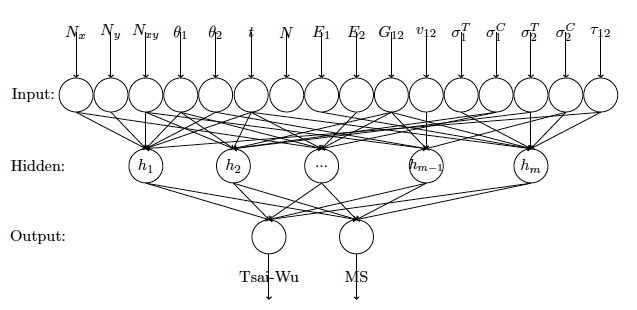
\includegraphics[width=0.9\textwidth]{fig/a0_figure_ann_for_clt_architecture.png}
		\caption{用于层合材料强度预测的神经网络}
	\end{figure}
\end{frame}

\note{
	根据上面的模型我们设计了以下的神经网络来预测层合材料的强度,
	该网络具有十六个输入参数:这16个参数是我们提取到的与层合材料结构有关的参数。
	两个输出,是不同的强度指标。

	To calculate the Based on the general neural network architecture, we proposed the
	following structure to predict the strength of angle ply structure. There
	are two outputs, which are tsai wu strength ratio, and maximum strength
	ratio.
	There are 16 inputs, which are consist of four parts:
	the first part is the loading that imposed on the laminate, Nx, Ny, Nxy
	the second part is the sequence of the angle ply laminate, which are two
	ply oritenation, ply thickness, and the number of plies.
	the third part is the four engineering  constants, E1,E2,G12, v12
	Traverse elastic modulus 
	Major Poisson's ratio 
	Shear modulus 
	the fourth part is five constants about the failure properties of the material: 
}

\begin{frame}{研究方法 }
	\begin{figure}
		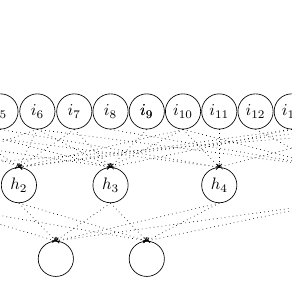
\begin{tikzpicture}
	[ p/.style={ draw=none, fill=none}, 
	  remember picture, 
	  net/.style={ matrix of nodes, nodes={ draw, circle, inner sep=7.5pt },
	  nodes in empty cells,
	  column sep=-10.5pt,
	  row sep=0.8cm, 
	  }
	]
	\useasboundingbox (-1.5,-1.1) rectangle (1.5,2);
	\scope[transform canvas={scale=0.6}]
\matrix[net] (mat)
{
		  & |[p]| &  & |[p]| &  & |[p]| &  & |[p]| &  & |[p]| &  & |[p]| &  & |[p]| &  & |[p]| &  &
			|[p]| &  & |[p]| &  & |[p]| &  & |[p]| &  & |[p]| &  & |[p]| &  & |[p]| &  & |[p]|    \\
	 |[p]| & |[p]| & |[p]| &  |[p]| &        & |[p]| & |[p]| & |[p]| &|[p]| &       & |[p]| &  |[p]| & |[p]| &
	 |[p]| &       & |[p]| &  |[p]| &  |[p]| & |[p]| & |[p]| &       &|[p]| & |[p]| & |[p]| & |[p]|
		   & |[p]| &       &  |[p]| &  |[p]| & |[p]| & |[p]| & |[p]| &|[p]| \\ 
	 |[p]| &  |[p]| & |[p]|  &  |[p]| & |[p]|  &  |[p]| &  |[p]| &  |[p]| & |[p]| & |[p]| & |[p]| &       & |[p]|
		   &  |[p]| & |[p]|  &  |[p]| &        &  |[p]| &  |[p]| &  |[p]| & |[p]| & |[p]| & |[p]| & |[p]| &     |[p]|
		   &  |[p]| & |[p]|  &  |[p]| & |[p]|  &  |[p]| &  |[p]| &  |[p]| \\ 
	  };
	  \node at (mat-1-1.base)  {$i_1$};
	  \node at (mat-1-3.base)  {$i_2$};
	  \node at (mat-1-5.base)  {$i_3$};
	  \node at (mat-1-7.base)  {$i_4$};
	  \node at (mat-1-9.base)  {$i_5$};
	  \node at (mat-1-11.base)  {$i_6$};
	  \node at (mat-1-13.base)  {$i_7$};
	  \node at (mat-1-15.base)  {$i_8$};
	  \node at (mat-1-17.base)  {$i_9$};
	  \node at (mat-1-17.base)  {$i_9$};
	  \node at (mat-1-19.base)  {$i_{10}$};
	  \node at (mat-1-21.base)  {$i_{11}$};
	  \node at (mat-1-23.base)  {$i_{12}$};
	  \node at (mat-1-25.base)  {$i_{13}$};
	  \node at (mat-1-27.base)  {$i_{14}$};
	  \node at (mat-1-29.base)  {$i_{15}$};
	  \node at (mat-1-31.base)  {$i_{16}$};

	  \node at (mat-2-5.base)  {$h_1$};
	  \node at (mat-2-10.base) {$h_2$};
	  \node at (mat-2-15.base) {$h_3$};
	  \node at (mat-2-21.base) {$h_4$};
	  \node at (mat-2-27.base) {$h_5$};
		 \foreach \a in {1,3,5,7,9,11,31}{
				\draw[->,dotted] (mat-1-\a.south) -- (mat-2-5.north);
			 }
		 \foreach \a in {5,7,11,13,19,25,27}{
				\draw[->,dotted] (mat-1-\a.south) -- (mat-2-10.north);
			 }
		 \foreach \a in {1,7,11,13,17,19,25}{
				\draw[->,dotted] (mat-1-\a.south) -- (mat-2-15.north);
			 }
		 \foreach \a in {5,9,19,21,29}{
				\draw[->,dotted] (mat-1-\a.south) -- (mat-2-21.north);
			 }
		 \foreach \a in {11,15,19,23,27,29,31}{
				\draw[->,dotted] (mat-1-\a.south) -- (mat-2-27.north);
			 }
		 \foreach \c in {5,10,15,21,27}{
			\foreach \d in {12,17}{
				\draw[->,dotted] (mat-2-\c.south) -- (mat-3-\d.north);
			}
 }
 \endscope
\end{tikzpicture}

		\caption{材料预测模型}
		\label{fig:example}
	\end{figure}
	\begin{table}
		\centering
		\caption{The binary representation of Figure \ref{fig:example}.
		}
		\begin{adjustbox}{width=0.8\textwidth}
		\begin{tabular}{l|cccc cccc cccc cccc | cc}
			\toprule
				 Nodes  & $i_1$ & $i_2$ & $i_3$ & $i_4$ & $i_5$ & $i_6$ & $i_7$ & $i_8$ & $i_9$ & $i_{10}$ & $i_{11}$ & $i_{12}$ & $i_{13}$ & $i_{14}$ & $i								_{15}$ & $i_{16}$ & f & f\\
			\midrule
				   	$h_1$ & 1  & 1 & 1  & 1  & 1 & 1 & 0 & 0  & 0 & 0 & 0 & 0  & 0 & 0  & 1 & 1 & 0 & 0\\
					$h_2$ & 0  & 1 & 1  & 1  & 0 & 0 & 0 & 1  & 0 & 0 & 1 & 1  & 0 & 0  & 0 & 0 & 1 & 1\\
					$h_3$ & 1  & 0 & 0  & 1  & 0 & 1 & 1 & 0  & 1 & 1 & 0 & 0  & 1 & 0  & 0 & 0 & 0 & 0\\
					$h_4$ & 0  & 0 & 1  & 0  & 1 & 0 & 0 & 0  & 0 & 1 & 0 & 1  & 0 & 0  & 1 & 0 & 0 & 1\\
					$h_5$ & 0  & 0 & 0  & 0  & 0 & 1 & 0 & 1  & 0 & 1 & 0 & 1  & 0 & 1  & 1 & 1 & 0 & 1\\
			\bottomrule
			\end{tabular}
		\end{adjustbox}
\end{table}



\end{frame}

\note{
	图八是我们随机产生的一个用于层合材料预测的网络结构,它有五个隐藏的神经元,每一个神经元
	与输入层的连接关系都是不同的,我们用下面的表哥来表示连接关系以及相对应的激活函数。
	在这个表哥中, }


\begin{frame}{研究方法 }
	\begin{figure}
	\centering
	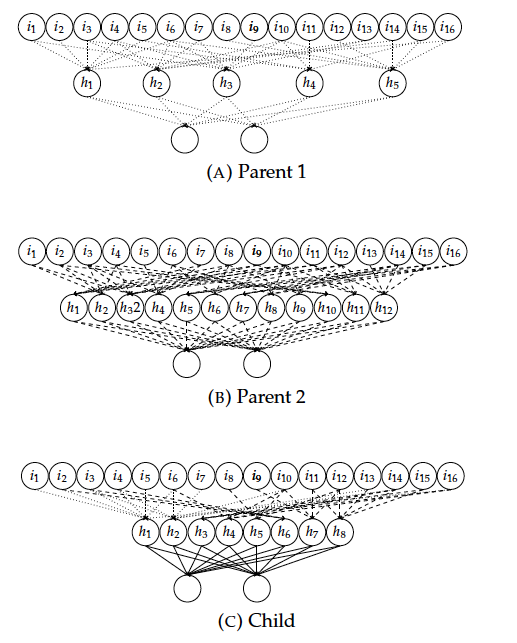
\includegraphics[scale=0.3]{fig/part3/interitance.png}
	\caption{基于遗传算法产生子神经网络 }
	\end{figure}
\end{frame}

\note{
	在这里我们给出的是根据使用遗传算法根据上一代的神经网络产生子神经网络的方式。产生的子神经网络
	会继承父神经网络的连接关系和激活函数。

	We also present the crossover operator about the neural network. child c
inherits the connection relationship part from parent 1 denoted by the darker
dashed lines,and the rest from parent 2 denoted by the gray dashed line}


\note{Since it is impossible to obtain enough training data from experiment,
therefore, we generate the training data by use of classical lamination theory and
failure theory. Table 11 shows part of our training data, in which the load
varys from -200 to 200 MP a for every component. the ply orientation varies
from -90 to 90. We use three different composite materail. The training data is
randomly sampled from this space. After obtain the two ouputs, we need
normalize the training data for the learning of the neural network.}

\begin{frame}{研究成果}
	\begin{columns}
		\begin{column}{0.6\textwidth}
			\begin{table}
	\centering
	\caption{Comparsion of Fully-connected Neural Network and GA-based Neural
	Network}
	\label{tab:simu}
		\resizebox{\textwidth}{!}{
	\begin{tabular}{ccc}
		\toprule
		Model     & Training Error & Validation Error   \\
		\midrule
		Fully-connected ANN &   0.051 & 0.050\\
		GA-based ANN       &   0.054 & 0.055\\
		\bottomrule
	\end{tabular}
}
\end{table}

		\end{column}
	\end{columns}
	\begin{center}
		\begin{itemize}
			\item Huiyao Zhang, Atsushi Yokoyama. 2021. Predicting Strength Ratio of Laminated Composite Material with Evolutionary
				Artificial Neural Network. International Journal of Advanced Computer Science and Applications, 12(6): 11‑18.
		\end{itemize}
	\end{center}
\end{frame}

\note{
 为了验证所推荐的网络结构和全连接神经网络在材料性能预测的差异,我们同时训练了一个全连接的
 神经网络。通过观察实验结果可以发现,演化神经网络在training error和validation
 error两个指标上都比全连接神经网络有更好的数据表现。并把我们的基于数据驱动的层合材料强度预测的研究成果发表在计算机类
 的期刊上。 

We also trained a neural network which has the same architecture as the neural
network that we obtained from genetic algorithm. The only difference is that
neurons in the hidden layer are fully connected with the inputs.
}

\begin{frame}{\hfill}
	\begin{tikzpicture}
		%\draw (1,1) grid (10,10);
		\draw[blue,dashed] (4,5) -- (6,4);
		\draw[blue,dashed] (6,4) -- (8,6);
		\draw[blue,dashed] (8,6) -- (9,5);
		\draw[blue,dashed] (9,5) -- (11,8);
		\draw[blue,dashed] (2,3) -- (4,5);
		\draw[blue,dashed] (2,3.5) -- (4,5.5);
		\draw[blue,dashed] (4,5.5) -- (6,4.5);
		\draw[blue,dashed] (6,4.5) -- (8,6.5);
		\draw[blue,dashed] (8,6.5) -- (9,5.5);
		\draw[blue,dashed] (9,5.5) -- (11,8.5);
		\node at (8,5) {\textcolor{blue}{\Huge{谢谢}}};
	\end{tikzpicture}
\end{frame}


\end{document}



